%%%%%%%%%%%%%%%%%%%%%%%%%%%%%%%%%%%%%%%%%
% baposter Landscape Poster
% LaTeX Template
% Version 1.0 (11/06/13)
%
% baposter Class Created by:
% Brian Amberg (baposter@brian-amberg.de)
%
% This template has been downloaded from:
% http://www.LaTeXTemplates.com
%
% License:
% CC BY-NC-SA 3.0 (http://creativecommons.org/licenses/by-nc-sa/3.0/)
%
%%%%%%%%%%%%%%%%%%%%%%%%%%%%%%%%%%%%%%%%%

%----------------------------------------------------------------------------------------
%	PACKAGES AND OTHER DOCUMENT CONFIGURATIONS
%----------------------------------------------------------------------------------------

\documentclass[landscape,a0paper,fontscale=0.25]{baposter} % Adjust the font scale/size here

\usepackage{graphicx} % Required for including images
\usepackage{graphics}

\graphicspath{{figures/}} % Directory in which figures are stored

\usepackage{amsmath} % For typesetting math
\usepackage{amssymb} % Adds new symbols to be used in math mode
\usepackage{tikz}
\usetikzlibrary{shapes,arrows, decorations}
\usepackage{booktabs} % Top and bottom rules for tables
\usepackage{enumitem} % Used to reduce itemize/enumerate spacing
\usepackage{palatino} % Use the Palatino font
\usepackage[font=small,labelfont=bf]{caption} % Required for specifying captions to tables and figures

\usepackage{multicol} % Required for multiple columns
\setlength{\columnsep}{1.5em} % Slightly increase the space between columns
\setlength{\columnseprule}{0mm} % No horizontal rule between columns


\newcommand{\compresslist}{ % Define a command to reduce spacing within itemize/enumerate environments, this is used right after \begin{itemize} or \begin{enumerate}
\setlength{\itemsep}{1pt}
\setlength{\parskip}{0pt}
\setlength{\parsep}{0pt}
}


\begin{document}

\begin{poster}
{
headerborder=closed, % Adds a border around the header of content boxes
colspacing=1em, % Column spacing
columns=3,
bgColorOne=white, % Background color for the gradient on the left side of the poster
bgColorTwo=white, % Background color for the gradient on the right side of the poster
borderColor=red, % Border color
headerColorOne=black, % Background color for the header in the content boxes (left side)
headerColorTwo=red, % Background color for the header in the content boxes (right side)
headerFontColor=white, % Text color for the header text in the content boxes
boxColorOne=white, % Background color of the content boxes
textborder=roundedleft, % Format of the border around content boxes, can be: none, bars, coils, triangles, rectangle, rounded, roundedsmall, roundedright or faded
eyecatcher=true, % Set to false for ignoring the left logo in the title and move the title left
headerheight=0.1\textheight, % Height of the header
headershape=roundedright, % Specify the rounded corner in the content box headers, can be: rectangle, small-rounded, roundedright, roundedleft or rounded
headerfont=\Large\bf\textsc, % Large, bold and sans serif font in the headers of content boxes
%textfont={\setlength{\parindent}{1.5em}}, % Uncomment for paragraph indentation
linewidth=2pt % Width of the border lines around content boxes
}
%----------------------------------------------------------------------------------------
%	TITLE SECTION 
%----------------------------------------------------------------------------------------
%
{
\includegraphics[height=4em]{UWlogo_fl_4c.png}} % First university/lab logo on the left
{\textsc{Data Analysis with Topic Models for Communications Researchers}}%\vspace{0.5em}} % Poster title
{\normalsize\textsc{Frederick Boehm (fred.boehm@wisc.edu), Department of Statistics, 
University of Wisconsin-Madison}} % Author names and institution
{
\includegraphics[height=4em]{UWCrest_4c.png}} % Second university/lab logo on the right

%----------------------------------------------------------------------------------------
%	OBJECTIVES
%----------------------------------------------------------------------------------------

\headerbox{Abstract}{name=abstract,column=0,row=0}{

We introduce topic modeling as a tool when analyzing textual data. We illustrate our methods with analyses of New York Times transcripts and tweets from three days in March 2016. We argue that such analyses will be useful in mass communications and journalism research. These methods are especially useful for identifying topics, or themes, in large collections of texts, when reading each piece individually is impractical.




\vspace{0.3em} % When there are two boxes, some whitespace may need to be added if the one on the right has more content
}

%----------------------------------------------------------------------------------------
%	INTRODUCTION
%----------------------------------------------------------------------------------------

\headerbox{Introduction}{name=introduction,column=0,below=abstract}{

Social media users flood us with tweets, status updates, and blog posts. Data analysis with topic models enable researchers to identify themes, or topics, in a collection of texts. We present results from separate analyses of 1) New York Times articles from March 19, 20, and 21, 2016 and 2) a collection of tweets (from Twitter) from the same three days. Our manuscript contains computing code to reproduce our findings.

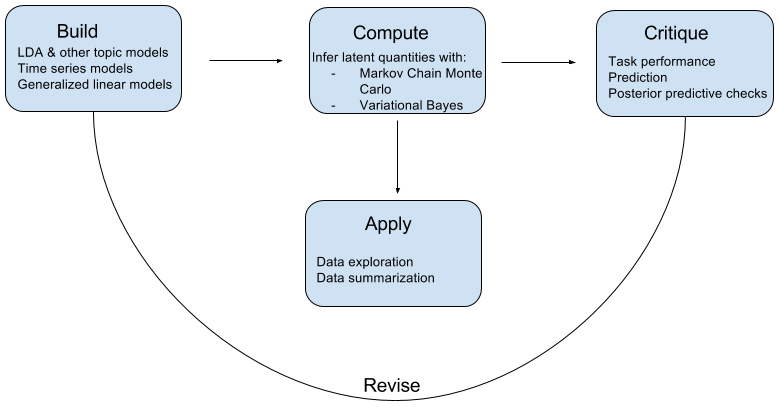
\includegraphics[scale = 0.32]{../box-blei-loop2.png}

}




%----------------------------------------------------------------------------------------
%	RESULTS 1
%----------------------------------------------------------------------------------------


%----------------------------------------------------------------------------------------
%	REFERENCES
%----------------------------------------------------------------------------------------

\headerbox{References}{name=references,column=1,span=2,above=bottom}{

\renewcommand{\section}[2]{\vskip 0.05em} % Get rid of the default "References" section title
%\nocite{*} % Insert publications even if they are not cited in the poster
\small{ % Reduce the font size in this block
\bibliographystyle{unsrt}
\bibliography{../twitter.bib} % Use sample.bib as the bibliography file
}}

%----------------------------------------------------------------------------------------
%	FUTURE RESEARCH
%----------------------------------------------------------------------------------------



%----------------------------------------------------------------------------------------
%	CONCLUSION
%----------------------------------------------------------------------------------------


%----------------------------------------------------------------------------------------
%	MATERIALS AND METHODS
%----------------------------------------------------------------------------------------

\headerbox{Methods}{name=method,column=0,below=introduction, above=bottom}{ % This block's bottom aligns with the bottom of the conclusion block
\begin{enumerate}
\item Fit latent Dirichlet allocation (LDA) models, separately, to 1) our collection of tweets and 2) our collection of print media articles from the New York Times
\item Visualized the topic modeling results with word clouds 
\item Assessed resulting topics for coherence
\end{enumerate}

}

%----------------------------------------------------------------------------------------
%	RESULTS 2
%----------------------------------------------------------------------------------------
\headerbox{Results}{name=results2,column=1,span=2,row=0}{ 

\begin{multicols}{2}

\begin{center}
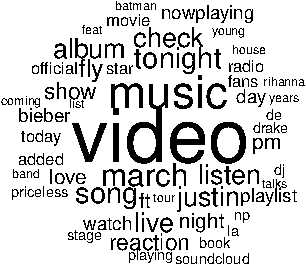
\includegraphics[scale = 0.8]{../lda-tutorial-2016_files/figure-latex/tw-wordcloud1-4.pdf}
\captionof{figure}{Word cloud for one topic (from a 20-topic model) of tweets from March 19, 20, and 21, 2016.}


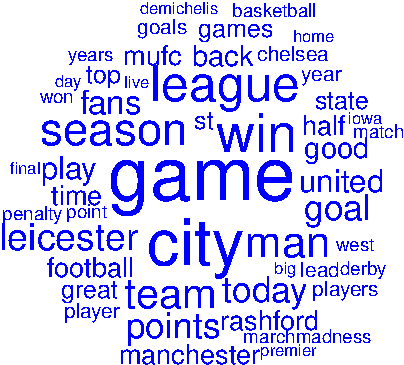
\includegraphics[scale = 0.8]{../lda-tutorial-2016_files/figure-latex/tw-wordcloud1-3.pdf}
\captionof{figure}{Word cloud for one topic (from a 20-topic model) of tweets from March 19, 20, and 21, 2016.}
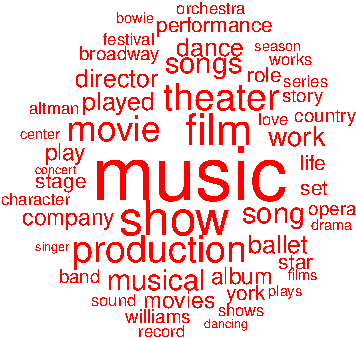
\includegraphics[scale = 0.8]{../lda-tutorial-2016_files/figure-latex/wordcloud1-1.pdf}
\captionof{figure}{Word cloud for one topic (from a 20-topic model) of New York Times articles from March 19, 20, and 21, 2016.}



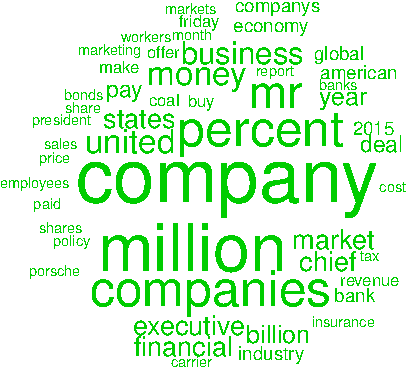
\includegraphics[scale = 0.6]{../lda-tutorial-2016_files/figure-latex/wordcloud1-2.pdf}
\captionof{figure}{Word cloud for one topic (from a 20-topic model) of New York Times articles from March 19, 20, and 21, 2016.}
\end{center}
\end{multicols}

}

\headerbox{Discussion}{name=discussion,column=1,span=2,below=results2, above=references}{
From the word clouds above, and those not shown, we find differences between the topics of discussion on Twitter and the topics in the New York Times. For instance, we find in the tweets an entire topic that deals with sports (with an emphasis on soccer) and another topic that involves music and entertainment. The New York Times analysis yields topics that match many of the newspaper sections. The two topics above might be called "Music" and "Travel \& Adventure".


} %end discussion

%----------------------------------------------------------------------------------------


\end{poster}

\end{document}